\section{Performance Modeling}
\label{sec:performance-modeling}

In this section we describe the performance model used to analyze the target system. We will follow the widely adopted modeling approach suggested in \cite{leemis2006discrete}, which consists in (i) goals and objectives (ii) conceptual model (iii) specification model (iv) computational model (v) verification and (vi) validation.


% %
% GOALS AND OBJECTIVES
% %
\subsection{Goals and Objectives}
The main goals of simulation are about system tuning.
In particular, we propose to determine with a $95\%$ level of confidence
\begin{itemize}
	\item the response time as a function of the threshold $S$,
	\item the throughput as a function of the threshold $S$,
	\item the distribution of the response time when $S=N$ and
	\item the threshold of the off-loading policy that minimizes the response time.
\end{itemize}


% %
% CONCEPTUAL MODEL
% %
\subsection{Conceptual Model}
The conceptual model of the target system is depicted in Figure~\ref{fig:conceptual-model}.

\begin{figure}
	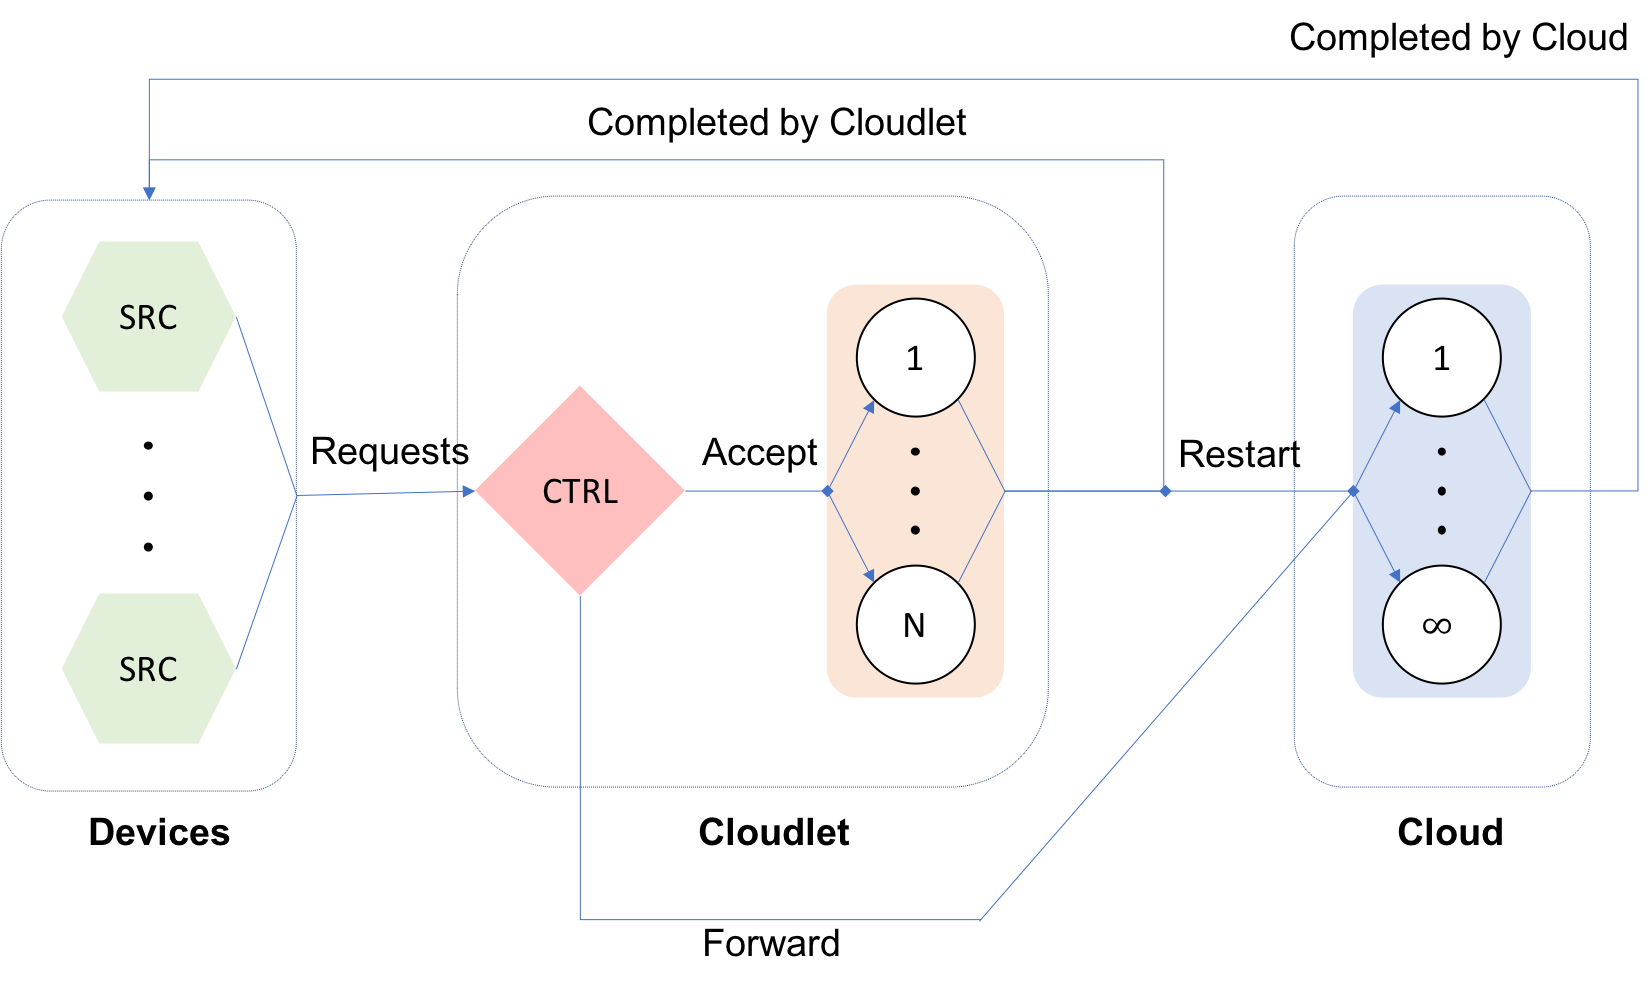
\includegraphics[width=\columnwidth]{fig/conceptual-model}
	\caption{Conceptual model.}
	\label{fig:conceptual-model}
\end{figure}

\paragraph{State space}
The state space $S$ of a system is a comprehensive characterization of the system. Each state $s \in S$ is a comprehensive characterization of the system in a given instant of time.
The state space of the whole system is represented by the state space of its subsystems:

\begin{itemize}
	\item Cloudlet: $S_{clt} := \{(n_{clt,1},n_{clt,2})\in \mathcal{N}^{2}: n_{clt,1}+n_{clt,2}\leq N\}$, where $n_{clt,j}$ is the population of tasks belonging to the $j$-th class within the Cloudlet.
	
	\item Cloud: $S_{cld} := \{(n_{cld,1},n_{cld,2})\in \mathcal{N}^{2}\}$, where $n_{cld,j}$ is the population of tasks belonging to the $j$-th class within the Cloud.
\end{itemize}

\paragraph{Events space}
An event is an occurrence that could change the state of the system at the event time, according to the event type.
We consider the following events:

\begin{itemize}
	\item $A_{clt,j}$: a task belonging to the $j$-th class arrives to the Cloudlet.
	
	\item $A_{cld,j}$: a task belonging to the $j$-th class arrives to the Cloud.

	\item $C_{clt,j}$: a task belonging to the $j$-th class is completed by the Cloudlet.
	
	\item $C_{cld,j}$: a task belonging to the $j$-th class is completed by the Cloud.
	
	\item $R_{2}$: a task belonging to the $2^{nd}$ class is stopped in the Cloudlet and restarted in the Cloud.
\end{itemize}

% %
% SPECIFICATION MODEL
% %
\subsection{Specification Model}

\paragraph{Statistical specifications}
Tasks belonging to the $j$-th class arrive to the system according to an exponential arrival process with rate $ \lambda_{j}$.
The Cloudlet serves tasks belonging to the $j$-th class according to an exponential service process with rate $\mu_{clt,j}$; the Cloud serves tasks belonging to the $j$-th class according to an exponential service process with rate $\mu_{cld,j}$.
We assume that 
(i) $\mu_{clt,i}>\mu_{cld,i}\ \forall i=1,2$ and
(ii) the setup time $T_{setup}$ is exponentially distributed with expected value $E[T_{setup}]$.

In particular, we consider values shown in Equations~\ref{eqn:statistical-specifications}.

\begin{equation} 
\begin{split}
\lambda_{1}  &=6.00\;tasks/sec \\
\lambda_{2}  &=6.25\;tasks/sec \\
\mu_{clt,1}  &=0.45\;tasks/sec \\
\mu_{clt,2}  &=0.27\;tasks/sec \\
\mu_{cld,1}  &=0.25\;tasks/sec \\
\mu_{cld,2}  &=0.22\;tasks/sec \\
E[T_{setup}] &=0.8\;sec \\
\end{split}
\label{eqn:statistical-specifications}
\end{equation}

\paragraph{Algorithmic specifications}
The \textit{off-loading policy} implemented by the \textit{Cloudlet controller (CTRL)} is defined in Algorithm~\ref{alg:offloading-policy}

\begin{algorithm}
	\SetAlgoLined
	\If{task of class 1}{
		\If{$n_{clt,1}=N$}{
			send to the Cloud
		} 
		\If{$n_{clt,1}+n_{clt,2}<S$}{
			accept on the Cloudlet
		} 
		\eIf{$n_{clt,2} > 0$}{
			accept on the Cloudlet, interrupt a $2^{nd}$ class task in the Cloudlet and restart it in the Cloud
		}{
		accept on Cloudlet
		}
	}
	\If{arrival of class 2}{
		\eIf{$n_{clt,1}+n_{clt,2}>=S$}{
			send to the Cloud
		}{
		accept on the Cloudlet
	}
	}
	\caption{Off-loading policy.}
	\label{alg:offloading-policy}
\end{algorithm}

% %
% ANALYTICAL MODEL
% %
\subsection{Analytical Model}
In this Section we will define and solve the \textit{analytical model} of the system.
%
In particular, we will first show the Markov Chain and flow balance equations for a very simple case, in order to introduce the reader to the structure of the chain with its critical states.
%
Then, we will cover the general case showing formulas of routing probabilities and performance metrics.
%
At the end, we will solve the target case explaining how we solve it.

The \textit{analytical model} is depicted in Figure~\ref{fig:analytical-model}, whose \textit{routing probabilities} are defined in Equation~\ref{eqn:routing-probabilities}.
The definition of routing probabilities relies on the following subsets of states $S_{clt,i} \subset S_{clt}$:

\begin{itemize}
	\item $S_{clt,1}$:  a task belonging to the $1^{st}$ class is accepted in the Cloudlet.
	
	\begin{equation}
	S_{clt,1} := \{(n_{clt,1},n_{clt,2})\in S_{clt} : n_{clt,1}+n_{clt,2}<N \vee n_{clt,2}>0\}
	\end{equation}
	
	\item $S_{clt,2}$: a task belonging to the $2^{nd}$ class is accepted in the Cloudlet.
	
	\begin{equation}
	S_{clt,2} := \{(n_{clt,1},n_{clt,2})\in S_{clt} : n_{clt,1}+n_{clt,2}<N \wedge n_{clt,2}<S\}
	\end{equation}
	
	\item $S_{clt,3}$: a task belonging to the $2^{nd}$ class is interrupted in the Cloudlet and it is restarted in the Cloud.
	
	\begin{equation}
	S_{clt,3} := \{(n_{clt,1},n_{clt,2})\in S_{clt} : n_{clt,1}+n_{clt,2}=N \wedge n_{clt,2}>0\}
	\end{equation}
\end{itemize}

\begin{figure}
	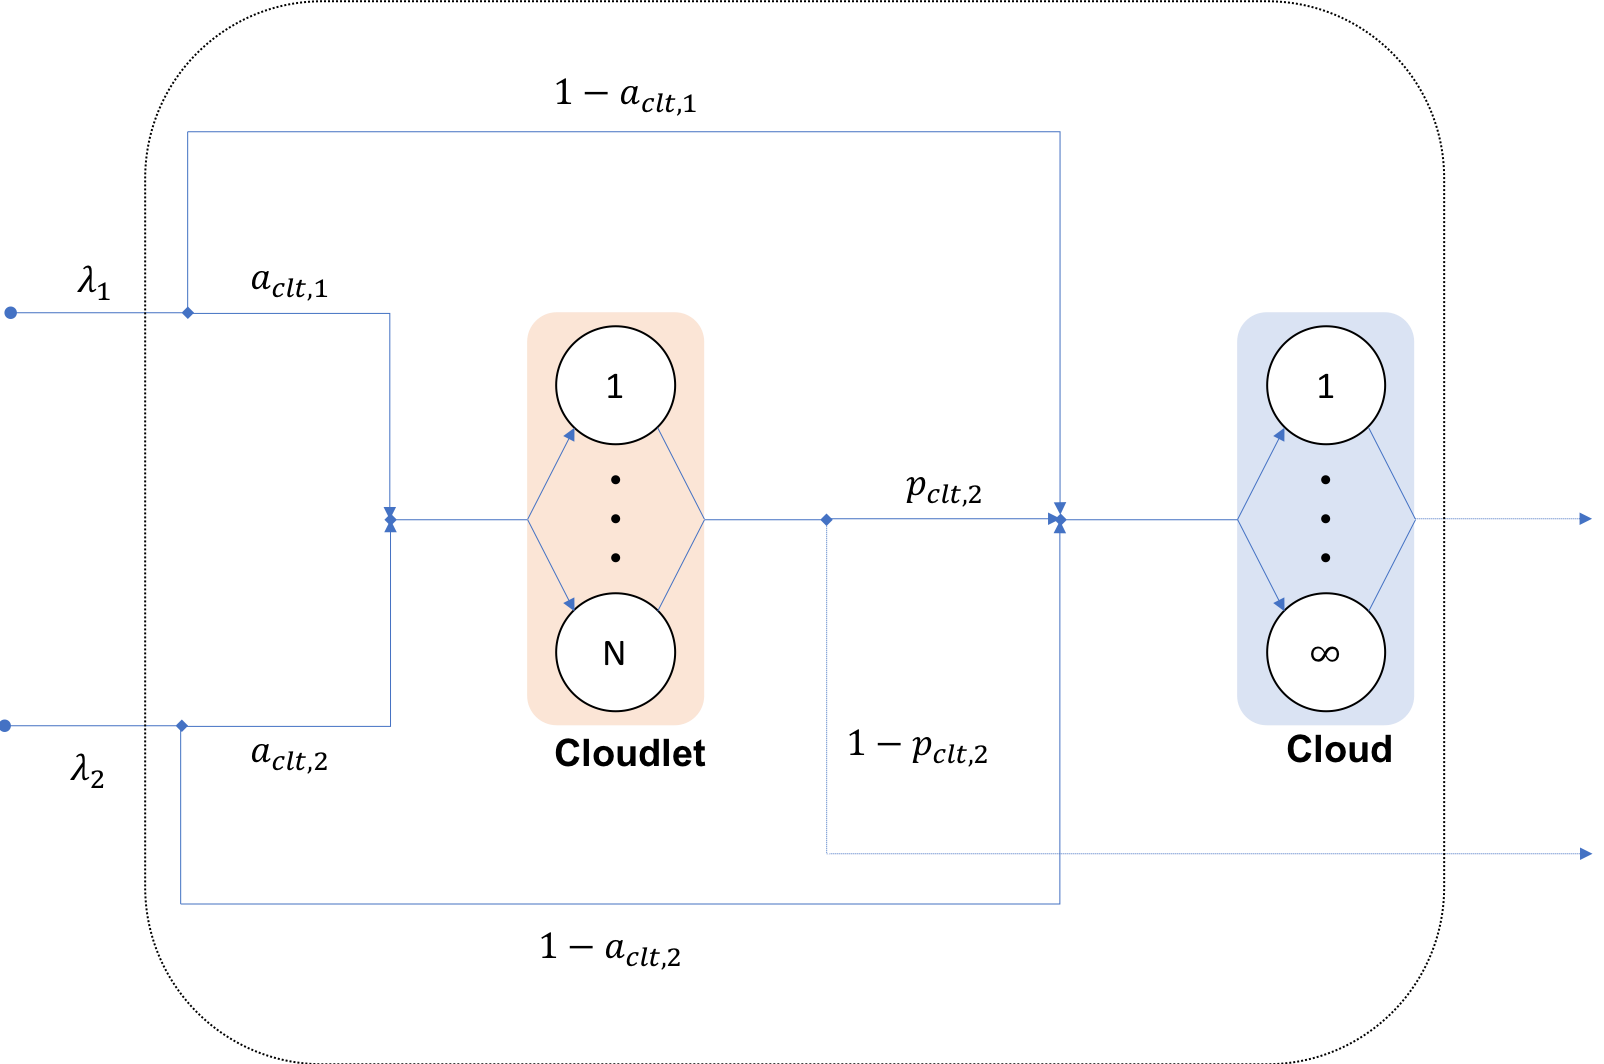
\includegraphics[width=\columnwidth]{fig/analytical-model}
	\caption{Analytical model.}
	\label{fig:analytical-model}
\end{figure}

\begin{equation} 
\begin{split}
a_{clt,1} & = \sum_{s\in S_{clt,1}} \pi_{s} \\
a_{clt,2} & = \sum_{s\in S_{clt,2}} \pi_{s} \\
r_{clt,2} & = \sum_{s\in S_{clt,3}} \pi_{s} \Big(\frac{\lambda_{2}}{\lambda_{1}+\lambda_{2}}\Big) \\
\end{split}
\label{eqn:routing-probabilities}
\end{equation}


\paragraph{Markov Chain}
Assuming Poisson arrivals and exponential services, we can determine the Markov Chain whose resolution allows us to compute the routing probabilities shown in Equation~\ref{eqn:routing-probabilities}.

In Figure~\ref{eqn:analytical-model-markov} we show the Markov Chain with the associated flow balance equations listed in Equation~\ref{eqn:analytical-model-markov}.
For sake of simplicity, we consider here the simple case with $N=S=2$ in order to (i) give an idea of the system of equations to be solved and (ii) graphically recognize the critical states. In fact, the representation fo the Markov Chain and the associated equations would be inpractical for the case $N=S=20$, due to the combinatorial explosion of the state space.

In the considered simple case, the critical states are:

\begin{itemize}
	\item $(2,0)$: every arrival is forwarded to the Cloud;
	
	\item $(1,1)$: every arrival belonging to class 1 is accepted in Cloudlet, causing the restart in Cloud of the serving task belonging to class 2; whilst every arrival belonging to class 2 is forwarded to Cloud;
	
	\item $(0,2)$: every arrival belonging to class 1 is accepted in Cloudlet, causing the restart in Cloud of a random serving task of Class 2; whilst every arrival belonging to class 2 is forwarded to Cloud;
\end{itemize}

\begin{figure}
	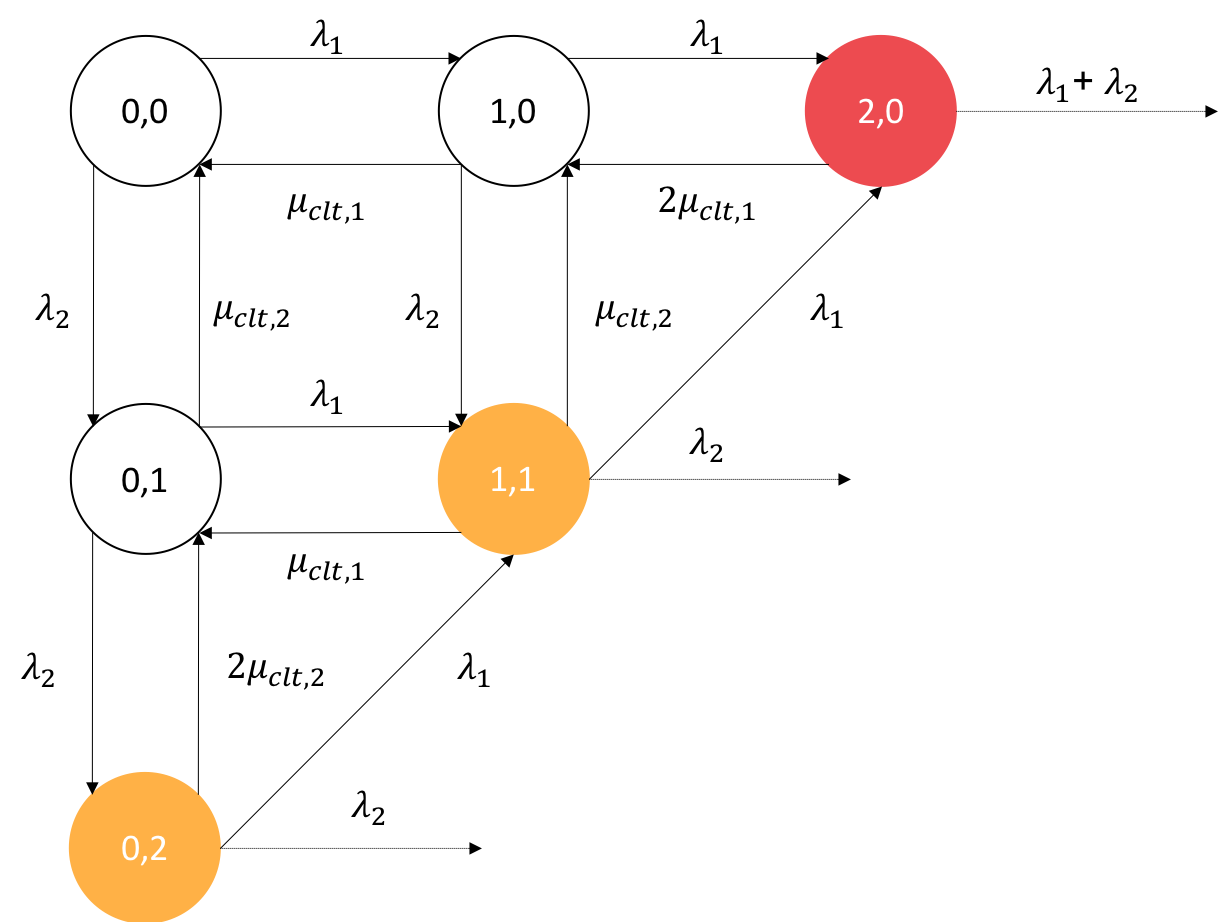
\includegraphics[width=\columnwidth]{fig/analytical-model-markov}
	\caption{Markov Chain with $N=2$ and $S=2$.}
	\label{fig:analytical-model-markov}
\end{figure}

\begin{equation} 
\begin{split}
\pi_{0,0}(\lambda_{1}+\lambda_{2})& = \pi_{1,0}\mu_{clt,1}+\pi_{0,1}\mu_{clt,2} \\
\pi_{0,1}(\lambda_{1}+\lambda_{2}+\mu_{clt,2}) & = \pi_{0,0}\lambda_{2}+\pi_{1,1}\mu_{clt,1}+\pi_{0,2}2\mu_{clt,2} \\
\pi_{1,0}(\lambda_{1}+\lambda_{2}+\mu_{clt,1}) & = \pi_{0,0}\lambda_{1}+\pi_{1,1}\mu_{clt,2}+\pi_{2,0}2\mu_{clt,1} \\
\pi_{1,1}(\lambda_{1}+\mu_{clt,1}+\mu_{clt,2}) & = \pi_{0,1}\lambda_{1}+\pi_{1,0}\lambda_{2}+\pi_{0,2}\lambda_{1} \\
\pi_{0,2}(\lambda_{1}+2\mu_{clt,2}) & = \pi_{0,1}\lambda_{2} \\
\pi_{2,0}2\mu_{clt,1} & = \pi_{1,0}\lambda_{1}+\pi_{1,1}\lambda_{1} \\
1 & = \pi_{0,0}+\pi_{0,1}+\pi_{1,0}+\pi_{1,1}+\pi_{0,2}+\pi_{2,0}\\
\end{split}
\label{eqn:analytical-model-markov}
\end{equation}

\paragraph{Accepted Workload}
Given the routing probabilities we can determine the following \textit{accepted workloads}:

\begin{itemize}
	\item Cloudlet: arrivals of tasks belonging to $j$-th class accepted in Cloudlet:
	\begin{equation}
	\lambda_{clt,j} = a_{clt,j}\lambda_{j}
	\end{equation}
	
	\item Cloud: arrivals of tasks belonging to $j$-th class forwarded to Cloud:
	\begin{equation}
	\lambda_{cld,j} = (1-a_{clt,j})\lambda_{j}
	\end{equation}
	
	\item Preemption: tasks belonging to $2$-nd class preempted in Cloudlet and restarted in Cloud:
	\begin{equation}
	\lambda_{p} = r(\lambda_{1}+\lambda_{2})
	\end{equation}
\end{itemize}

\paragraph{Performance metrics}
Given the accepted workloads we can determine the following \textit{performance metrics for classed tasks in each subsystem}:

\begin{itemize}
	\item $1^{st}$ class in Cloudlet:
	\begin{equation} 
	\begin{split}
	E[T_{clt,1}] &= \frac{1}{\mu_{clt,1}} \\
	E[N_{clt,1}] &= \lambda_{clt,1}E[T_{clt,1}] \\
	\end{split}
	\end{equation}

	\item $2^{nd}$ class in Cloudlet:
	\begin{equation} 
	\begin{split}
	E[T_{clt,2}] &= \frac{1}{\mu_{clt,2}} \\
	E[N_{clt,2}] &= \lambda_{clt,2}E[T_{clt,2}]-\psi\lambda_{p}E[T_{clt,2}] \\
	\end{split}
	\end{equation}
	
	\item $1^{st}$ class in Cloud:
	\begin{equation} 
	\begin{split}
	E[T_{cld,1}] &= \frac{1}{\mu_{cld,1}} \\
	E[N_{cld,1}] &= \lambda_{cld,1}E[T_{cld,1}] \\
	\end{split}
	\end{equation}
	
	\item $2^{nd}$ class in Cloud (not preempted):
	\begin{equation} 
	\begin{split}
	E[T_{cld,2}]^{[NP]} &= \frac{1}{\mu_{cld,2}} \\
	E[N_{cld,2}]^{[NP]} &= \lambda_{cld,2}E[T_{cld,2}]^{[NP]} \\
	\end{split}
	\end{equation}
	
	\item $2^{nd}$ class in Cloud (preempted):
	\begin{equation} 
	\begin{split}
	E[T_{cld,2}]^{[P]} &= E[T_{clt,2}]+E[T_{setup}]+\psi E[T_{cld,2}]^{[NP]} \\
	E[N_{cld,2}]^{[P]} &= \lambda_{p}E[T_{cld,2}]^{[P]} \\
	\end{split}
	\end{equation}
	
	\item $2^{nd}$ class in Cloud (not preempted and preempted):
	\begin{equation} 
	\begin{split}
	E[T_{cld,2}] &= \sum_{m=NP,P}\frac{E[N_{cld,2}]^{[m]}}{E[N_{cld,2}]}E[T_{cld,2}]^{[m]} \\
	E[N_{cld,2}] &= \sum_{m=NP,P}E[N_{cld,2}]^{[m]} \\
	\end{split}
	\end{equation}
\end{itemize}

Then we can determine the following \textit{performance metrics for each subsystem}:

\begin{itemize}
	\item Cloudlet:
	\begin{equation} 
	\begin{split}
	E[T_{clt}] &= \sum_{j=1,2}\frac{E[N_{clt,j}]}{E[N_{clt}]}E[T_{clt,j}] \\
	E[N_{clt}] &= \sum_{j=1,2}E[N_{clt,j}] \\
	E[X_{clt}] &= \sum_{j=1,2}\lambda_{clt,j}-\lambda_{p} \\
	\end{split}
	\end{equation}
	
	\item Cloud:
	\begin{equation} 
	\begin{split}
	E[T_{cld}] &= \sum_{j=1,2}\frac{E[N_{cld,j}]}{E[N_{cld}]}E[T_{cld,j}] \\
	E[N_{cld}] &= \sum_{j=1,2}E[N_{cld,j}] \\
	E[X_{cld}] &= \sum_{j=1,2}\lambda_{cld,j}+\lambda_{p} \\
	\end{split}
	\end{equation}
\end{itemize}

Finally, we can determine the following \textit{performance metrics for the whole system}:

\begin{equation} 
\begin{split}
E[T] &= \sum_{i=cld,clt}\frac{E[N_{i}]}{E[N]}E[T_{i}] \\
E[N] &= \sum_{i=cld,clt}E[N_{i}] \\
E[X] &= \sum_{i=cld,clt}E[X_{i}] \\
\end{split}
\end{equation}

Thinking about the \textit{utilization of each subsystem}, the following hold true:

\begin{itemize}
	\item Cloudlet: simplifying our argument by assuming the whole incoming traffic belonging to the $1^{st}$ class served at the maximum rate (the best case), we can state that
	\begin{equation} 
	\rho_{clt} = \frac{\lambda_{1}+\lambda_{2}}{N\mu_{clt,1}}\rightarrow 0
	\end{equation}
	That is, the Cloudlet is not able to serve all traffic as it saturates.
	
	\item Cloud: as a queue with infinite resources, we can conclude that
	\begin{equation}
	\rho_{cld} \rightarrow 0
	\end{equation}
	That is, the Cloud can handle all requests as it never saturates.
\end{itemize}


\paragraph{Resolution}
Given the \textit{analytical model} depicted in Figure~\ref{fig:analytical-model}, the resolution of the Markov Chain for the case $S=N=20$ allows us to determine the routing probabilities and performance metrics shown at the end of this paragraph.

We solved the the \textit{analytical model} depicted in Figure~\ref{fig:analytical-model} leveraging (i) a \textit{Python script} that determines the transition matrix and the notable subsets of states, i.e. $S_{clt,1}$, $S_{clt,2}$ and $S_{clt,3}$, and (ii) a \textit{Matlab Live Script} that takes them as input and computes routing probabilities, accepted/preempted traffic and performance metrics.



% %
% COMPUTATIONAL MODEL
% %
\subsection{Computational Model}
The proposed simulator has been designed following the \textit{next-event simulation} paradigm and has been implemented as a \textit{Python} application. The full open source code is available in a public Github repository \cite{gmarciani-pydes}.
Representative examples of configuration and outputs are presented in Section~\ref{sec:usage}.

\paragraph{Configuration}
The simulation parameters can be fully configured with a YAML file loaded when the simulator starts up. In particular, the following parameters can be configured:

\begin{itemize}
	\item \textit{arrival process}: the user can configure the statistical distribution law and parameters of arrivals for both task classes. In this work, we consider the Exponential distribution, but any statistical distribution can be set.
	
	\item \textit{service process}: the user can configure the statistical distribution law and parameters of services for both task classes. In this work, we consider the Exponential distribution, but any statistical distribution can be set.
	
	\item \textit{setup time}: the user can configure the statistical distribution law and parameters of the setup time for both task classes. In this work, we consider a Deterministic setup time set to zero for the $1^{st}$ class and an Exponential setup time for the $2^{nd}$ class, but any statistical distribution can be set.
	
	\item \textit{Cloudlet dimension}: the user can configure the number of Cloudlet resources.
	
	\item \textit{Cloudlet threshold}: the user can configure the threshold for the restart condition of $2^{nd}$ class tasks in the Cloudlet.
	
	\item \textit{server selection policy}: the user can configure the policy adopted to select the $2^{nd}$ class task to interrupt in the Cloudlet when the threshold has been reached. In this work, we consider the Random selection, but the user can choose among Random, Ordered, Cyclic and Equity selection policies.
\end{itemize}

\paragraph{Randomization}
Random components are ruled by a custom \textit{multi-stream Lehmer generator} to generate pseudo-random events, whose parameters have been described in Section~\ref{sec:random-number-generation} and whose evaluation is presented in Section~\ref{sec:evaluation}.
The \textit{degree of randomization} has been improved by associating the random component the following processes to a dedicated stream of the pseudo-random number generator: arrival process of each task class, service process of each servant and server selection rule.
This strategy has been motivated by the fact that in a real case scenario we can assume the independence between (i) inter-classed workload, (ii) computational offer of distinct resources and (iii) selection strategies.

\paragraph{Event management}
Events are managed by a \textit{priority-queue based calendar} with the ability both to schedule and un-schedule events.
%
Even if both the initial and terminal state can have any possible value, we adopted the convention of initializing and terminating the system in the idle state $(0,0,0,0)$. In particular, the terminal state is reached via the well-known closed door technique driven by a stop time condition.
%
The calendar is initialized by scheduling the first arrival in the initialization phase. The submission of an arrival $a$ to the system could induce
(i) the scheduling of the corresponding completion event,
(ii) the scheduling of a new arrival, or
(iii) the unscheduling of a previously scheduled completion, i.e. interruption in Cloudlet.
%
The next-event calendar is implemented as priority queue, appropriately extended to manage scheduling/unscheduling of events and exclusion of impossible events, i.e. arrivals with occurrence time greater than the stop time.
%
The impossibility of events is managed by letting the calendar contain possible events only, which is the best approach when the event list is assumed to be very long.

\paragraph{Software Classes}
We provide here a short description of the main software classes involved in our simulator, in order to help the reader navigate through our code.

\begin{itemize}

	\item \textit{Simulation}: simulator entry-point, responsible to load and validate configurations, create the calendar of events, the statistics and the target system, show the real-time progress of the simulation, determine the duration of the simulation, write sampling files, reports and output results.
	
	\item \textit{Calendar}: calendar of events, implemented as a priority-queue with the ability to both schedule and unschedule events.
	
	\item \textit{System}: high level abstraction of the whole system, responsible to initialize the Cloudlet, initialize the Cloud, implement the Controller logic and update system-level classed/global metrics.
	
	\item \textit{Cloudlet}: represents the Cloudlet subsystem, responsible to handle events, select the task to interrupt according to the selection policy and update Cloudlet-level classed/global metrics.
	
	\item \textit{Cloud}: represents the Cloud subsystem, responsible to handle events and update Cloudlet-level classed/global metrics.
	
	\item \textit{RandomComponent}: represents a fully-customizable independent random process. In particular, the calendar and each subsystem receive as input an instance of this object in order to realize their own random logic.
	
	\item \textit{RndGen}: instance of a fully-customizable multi-stream Lehmer pseudo-random number generator.
	
	\item \textit{Stats}: abstraction encapsulating all metrics involved in the simulation, responsible to make it easy to update metrics during the simulation loop. In particular, each subsystem receives as input a reference to this singleton in order to centralize the management of performance metrics.
\end{itemize}


% %
% VERIFICATION
% %
\subsection{Verification}
The main goal of verification is to assess the consistency of the computational model with the specification model.
The verification has been carried out by evaluating the following consistency checks based on simulator logs and outputs:

\begin{itemize}
	\item \textbf{state consistency:} verifies the correctness of the system state evolution, i.e. state transitions;
	
	\item \textbf{arrival consistency:} verifies the correctness of arrivals ordering, i.e. tasks arrived before are served before;
	
	\item \textbf{service consistency:} verifies the correctness of service ordering, i.e. tasks with less service time leave the system before;
	
	\item \textbf{flow consistency:} verifies the correctness of flow trends, such as:
	
	\begin{equation}
	n_{clt,i}=a_{clt,i}-s_{clt,i}-c_{clt,i}
	\end{equation}
	\begin{equation}
	n_{cld,i}=a_{cld,i}+s_{cld,i}-c_{cld,i}
	\end{equation}
	\begin{equation}
	s_{clt,i}=s_{cld,i}
	\end{equation}
	
	where 
	$n_{j,i}$ is the population in the $j$-th subsystem belonging to $i$-th class of tasks, 
	$a_{j,i}$ is the number of arrivals to the $j$-th subsystem belonging to $i$-th class of tasks,
	$c_{j,i}$ is the number of completions in the $j$-th subsystem belonging to $i$-th class of tasks
	$s_{j,i}$ is the number of switches from/to the $j$-th subsystem belonging to $i$-th class of tasks\footnote{notice that $s_{j,1}=0\forall j=1,2$, as tasks belonging to class $C1$ cannot be switched from Cloudlet to Cloud.}.
	 
	\item \textbf{workload change consistency:} verifies the correctness of performance metrics variations in response to arrival/service rates variations. For example, we verified that the following hold true:
	
	\begin{equation}
		\mu_{cld,2}^{new} > \mu_{cld,2}^{old} \Rightarrow E[T_{sys,2}]^{new} > E[T_{sys,2}]^{old}
	\end{equation}
	\\
	and
	
	\begin{equation}
	S^{new} > S^{old} \Rightarrow E[N_{cld,2}]^{new} < E[N_{cld,2}]^{old}
	\end{equation}
\end{itemize}

% %
% VALIDATION
% %
\subsection{Validation}
It is well-known that model development should include a final validation step in order to assess the consistency of the model with the real system. 
%
As the simulation main purpose is insight, a widely adopted Turing-like technique is to place the computational model alongside with the real system and assess the consistency of performance indices.
%
Clearly, we cannot adopt this technique as we cannot compare the model with its real counterpart.
%
For this reason, we totally rely on the validation with respect to the analytical model. 
In Figure \ref{tbl:evaluation} we show the comparison between theoretical performance results, taken from the analytical model, and their experimental counterpart, taken from the simulator. 
The obtained results demonstrate that our simulator is a pretty reliable tool to conduct the performance analysis of the target system. Where the experimental values do not coincide with the theoretical ones, this is to be attributed to the adoption of the random selection of the tasks to be interrupted.